\chapter{Kinect--Framework}
\label{chap:Kinect}

\section{Microsoft Kinect SDK}
% Auflistung der Bereitgestellten Funktionen und Umfang des SDK-Toolkits

% \footnote{Microsoft Corporation (2012) \href{http://msdn.microsoft.com/en-us/library/hh973075.aspx}{\textit{DataStreams}} msdn.microsoft.com, Abgerufen Januar 03, 2013}

Das Kinect SDK von Microsoft stellt, wie zuvor bereits erw\"ahnt, die technische Schnittstelle zur Kinect zur Verf\"ugung. 
Dies sind zum einen die Programmierschnittstellen in den Sprachen C++, C\# und VB .net also auch die ben\"otigten Treiber 
und \glslink{Runtime Library}{Runtime Libraries}, die die Kommunikation mit dem Ger\"at erm\"oglichen. 
In der nachfolgenden Abbildung ist der Aufbau des SDK abgebildet.
\par\smallskip 
\begin{figure}[htb]
\centering
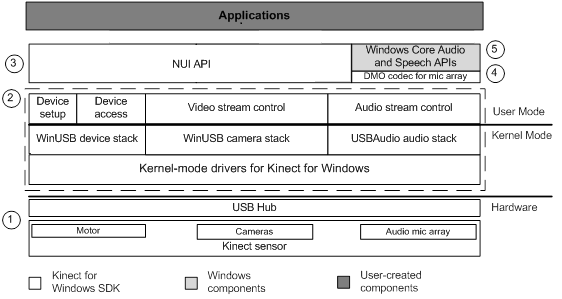
\includegraphics[width=0.8\textwidth]{img/04kapitel/sdk.png}
\caption[SDK Architektur]{SDK Architektur (Quelle: Microsoft Corp.\footnotemark[1])}
\label{fig:SDK Architecture}
\end{figure}
\footnotetext[1]{Microsoft Corp. (2012) \href{http://msdn.microsoft.com/en-us/library/jj131023.aspx}{\textit{SDK Architektur}} msdn.microsoft.com, Abgerufen Januar 03, 2013}
\par\smallskip 
Die Ebene 3 enth\"alt die Programmierschnittstelle. Mittels der \glslink{NUI}{NUI} \glslink{API}{API} kann auf die 
Datenstr\"ome, die die Kinect liefert zugegriffen werden. Von der Kinect werden hier vier Datenstr\"ome\footnotemark[2] geliefert: 
\begin{itemize}
  \item AudioStrom
  \item Farbstrom
  \item Tiefenstrom
  \item Infrarotstrom
\end{itemize}
\footnotetext[2]{Microsoft Corp. (2012) \href{http://msdn.microsoft.com/en-us/library/hh973075.aspx}{\textit{DataStreams}} msdn.microsoft.com, Abgerufen Januar 03, 2013}
\par\smallskip 
Auf Basis dieser Datensr\"ome kann eine Erkennung von Personen, Gesten und Sprachkommandos realisiert werden.
Dies ist jedoch nicht zwingend notwendig, da hier durch die M\"oglichkeit des Zugriffs auf einen Skelettstrom bereits, 
ohne diesen Transformationsschritt von Rohdaten zu einem Model, auf die Koordinaten eines Modells des menschlichen K\"orpers 
zugegriffen werden kann. Diese Komponente kann bis zu 2 Personen erkennen und die Modelle dieser Personen liefern\footnotemark[3].
Das Modell basiert auf 20 Punkten, die bestimmt K\"orperteile und -regionen abbilden. Dieses Modell ist in Abbildung~\ref{fig:skeleton} zu sehen.
\par\smallskip 
\begin{figure}[htb]
\centering
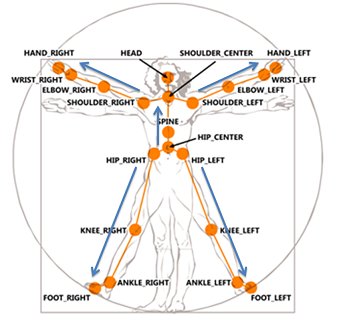
\includegraphics[width=0.8\textwidth]{img/04kapitel/skeleton.png}
\caption[Skeleton]{Skeleton (Quelle: Microsoft Corp.\footnotemark[3])}
\label{fig:skeleton}
\end{figure}
\footnotetext[3]{Microsoft Corp. (2012) \href{http://msdn.microsoft.com/en-us/library/jj131025.aspx}{\textit{Tracking Users with Kinect Skeletal Tracking}} msdn.microsoft.com, Abgerufen Januar 03, 2013}
\newpage
Auf dieser Basis wird es schon relativ leicht m\"oglich eine Gestensteuerung zu entwickeln. Weitere Beispiele f\"ur das Tracking bilden die 
Ausgabe des Kinect Explorer\footnotemark[4], einem Beispiel welches Teil des SDK ist und einer Visualisierung mittels \glslink{GEF}{GEF} in der 
Anwendung die im Rahmen dieser Arbeit entwickelt wird. In Abbildung~\ref{fig:kinectexplorer} ist die Visualisierung der Punkte im Kinect Explorer zu sehen, 
in Abbildung~\ref{fig:gef} die Darstellung in mit dem \glslink{GEF}{Graphical Editing Framework}.
\footnotetext[4]{Microsoft Corp. (2012) \href{http://msdn.microsoft.com/en-us/library/hh855378}{\textit{Kinect Explorer}} msdn.microsoft.com, Abgerufen Januar 03, 2013}
\par\smallskip 
\begin{figure}[htb]
\centering
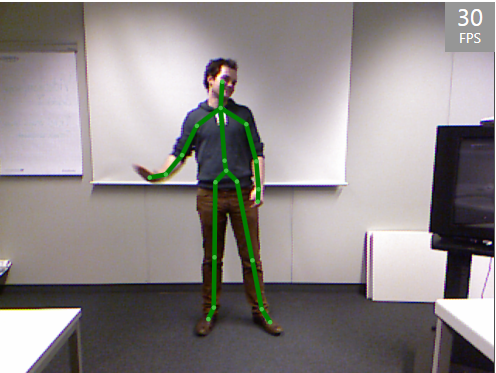
\includegraphics[width=0.8\textwidth]{img/04kapitel/kinectexplorer.png}
\caption[Kinect Explorer]{Kinect Explorer\footnotemark[4]}
\label{fig:kinectexplorer}
\end{figure}
\begin{figure}[!]
\centering
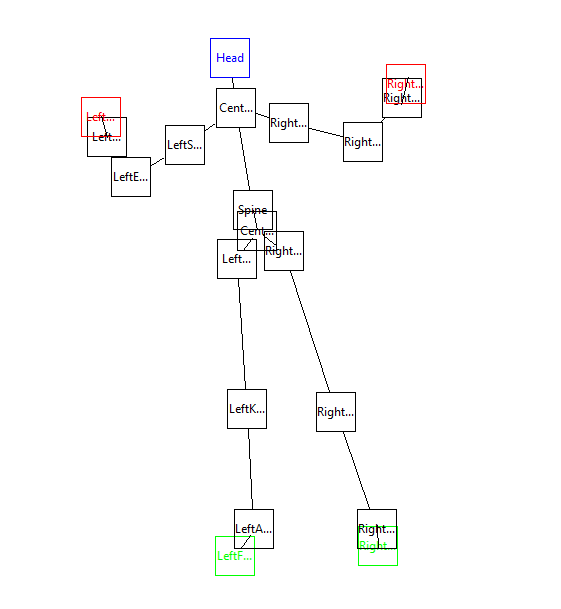
\includegraphics[width=0.8\textwidth]{img/04kapitel//gefeditor.png}
\caption[GEF Editor]{GEF Editor}
\label{fig:gef}
\end{figure}
\newpage
Au\ss erdem ist es auch unter Verwendung des SDK in mindestens Version 1.5 und einer \textit{Kinect for Windows} m\"oglich 
ein Gesicht und dessen Bewegungen zu erfassen\footnotemark[5]. Diese Funktion wird im ersten Teil dieser Arbeit jedoch noch keine Anwendung finden.
\footnotetext[5]{Microsoft Corp. (2012) \href{http://msdn.microsoft.com/en-us/library/jj130970.aspx}{\textit{Face Tracking}} msdn.microsoft.com, Abgerufen Januar 03, 2013}
\par\smallskip 
Zur Spracherkennung muss ebenfalls nicht notwendigerwei\ss e direkt der Audiostrom der Kinect analysiert werden. Mittels einer Speechengine kann auf Basis 
einer durch den Entwickler definierten Grammatik Sprache erkannt werden. Der Entwickler wird dann \"uber erkannte Kommandos mittels Events benachrichtigt. 

\section{Java Frameworks}
% Nutzung von Java begr\"unden etc.

Da die Entwicklung mit Java durchgef\"uhrt werden soll ist es notwendig einen \glslink{Wrapper}{Wrapper} f\"ur das Kinect SDK zu verwenden.
Hierzu existieren bereits diverse Frameworks die genau das erm\"oglichen.
Nachfolgend werden drei dieser Frameworks betrachtet und deren Nutzbarkeit im Rahmen dieser Arbeit evaluiert.
Abschlie\ss end wird ein Framework ausgew\"ahlt auf dessen Basis die Umsetzung dieser Arbeit erfolgen soll.
\par\smallskip 
Ziel dieser Arbeit ist die Umsetzung einer Gesten- und Sprachsteuerung. Daher sollte ein m\"oglichst einfacher Zugang zum Skelettstrom und der 
Spracherkennungskomponennte des Kinect SDK vorhanden sein. Eine Eigenentwicklung dieser Funktionen w\"urde den Rahmen dieser Arbeit bei weitem \"uberschreiten.


\subsection{OpenNI}
% Einf\"uhrende Worte zu Framework: Initiator und Startzeitpunkt des Projekts, aktuelle Version

\subsubsection{Beschreibung}
\gls{OpenNI}\footnotemark[7] ist der Name eines Industriekonsortiums dessen Ziel es ist, die Entwicklung und Standardisierung von Software und Hardware 
im Bereich der Natural User Interfaces.
Es wurde im November 2010 ins Leben gerufen und setzt sich aus verschiedenen großen Unternehmen zusammen. Dazu geh\"ort beispielsweise Primesense, 
welches selbst solche Ger\"ate entwickelt und vertreibt oder auch ASUS, welche in Kooperation mit Primesense die Xtion Pro\footnotemark[9] entwickelt haben und vertreiben.
Zusammen formen diese unter dem Namen OpenNI eine Non-Profit-Organisation.

\footnotetext[6]{OpenNI \href{http://www.openni.org/}{\textit{Home}} openni.org, Abgerufen Januar 04, 2013}
\footnotetext[7]{OpenNI \href{http://www.openni.org/organization/}{\textit{Organization}} openni.org, Abgerufen Januar 04, 2013}
\footnotetext[8]{OpenNI \href{http://www.openni.org/about/}{\textit{About}} openni.org, Abgerufen Januar 04, 2013}
\footnotetext[9]{Asus (Mai 2011) \href{http://www.asus.de/Multimedia/Motion_Sensor/Xtion_PRO/}{\textit{Xtion Pro}} aus.de, Abgerufen Januar 04, 2013}

\subsubsection{Technische Daten}

Durch OpenNI wird ein SDK und eine Plattform zur Verf\"ugung gestellt, mit der eine Verbindung mit verschiedenen Ger\"aten m\"oglich ist. Zu sehen ist der Aufbau in Abbildung~\ref{fig:opennisdk}.
Das SDK stellt eine Schnittstelle zu den grunds\"atzlichen Sensoren der Hardware und den davon generierten Datenstr\"omen dar.
Einzig der Audiostrom wird zum jetzigen Zeitpunkt noch nicht nutzbar.
Durch den Einsatz von \textit{Middleware Libraries} k\"onnen abstraktere Funktionen, wie das Tracking eines Skelettes abgebildet werden. Ein Beispiel 
hierf\"ur ist die Middleware Nite 2\footnotemark[10] von Primesense. Das SDK eignet sich grunds\"atzlich zur Nutzung verschiedener Ger\"ate, 
sofern Treiber verf\"ugbar sind, ist also nicht auf die Kinect festgelegt.
Eigene Anwendungen lassen sich mittels der API in C++ entwickeln. Außerdem werden \gls{Wrapper} Java und C\# bereitgestellt.
Zugriff auf das Mikrofonarray ist jedoch nicht gegeben und muss vom Benutzer selbst implementiert werden. 
Somit steht hier auch keine nutzbare Engine zur Spracherkennung zur Verf\"ugung.
Auch durch Middleware wird hier keine L\"osung geboten.

\begin{figure}[!]
\centering
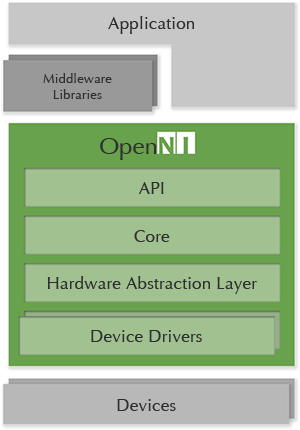
\includegraphics[width=0.4\textwidth]{img/04kapitel/OpenNI2_Architecture2.png}
\caption[Kinect Explorer]{Architektur des OpenNI SDK\footnotemark[8]}
\label{fig:opennisdk}
\end{figure}
\footnotetext[10]{OpenNI \href{http://www.openni.org/files/nite/}{\textit{Nite 2}} openni.org, Abgerufen Januar 04, 2013}

\subsubsection{Analyse der Anwendbarkeit}

Eine Java-Schnittstelle ist vorhanden. Das Skeleton-Tracking wird durch das SDK direkt nicht geboten, wird jedoch von einer Middleware zur Verf\"ugung gestellt, 
welche ebenfalls eine Java-Schnittstelle besitzt. Jedoch verf\"ugt dieses SDK nicht \"uber die M\"oglichkeit die Spracheingabe auf Muster zu untersuchen. Eine Spracherkennung ist also nicht geboten.

\newpage

\subsection{OpenKinect}

\subsubsection{Beschreibung}

OpenKinect\footnotemark[11] ist eine Open Source Community, die sich aus Personen zusammensetzt deren Interesse in der Entwicklung rund um die Kinect und \"ahnlichen Ger\"aten liegt.
Diese Community entwickelt derzeitig die Software libfreenect. Diese ist die Schnittstelle zur Kinect. Das Projekt ist allein durch seine Community getragen.

\subsubsection{Technische Daten}

OpenKinect ist in C geschrieben, stellt jedoch Wrapper f\"ur viele weitere Sprachen bereit\footnotemark[12], darunter auch Java. Außerdem sind Treiber f\"ur die Kinect enthalten.
Hiermit besteht Zugriff auf die, durch die Kinect gelieferten, Rohdaten.

\footnotetext[11]{OpenKinect \href{http://openkinect.org/wiki/Main_Page}{\textit{OpenKinect Mainpage}} openkinect.org, Abgerufen Januar 05, 2013}
\footnotetext[12]{Abschnitt Wrapper \href{http://openkinect.org/wiki/Main_Page}{\textit{OpenKinect Mainpage}} openkinect.org, Abgerufen Januar 05, 2013}

\subsubsection{Analyse der Anwendbarkeit}

Dieses Projekt bietet ebenfalls die M\"oglichkeit mittels Java auf die Kinect zuzugreifen. Jedoch sind auch hier bislang keine Erweiterungen verf\"ugbar. Hier stellt sich ebenfalls das Problem der nicht vorhanden Spracherkennung.


\subsection{jnect}
\label{subsec:jnect}

\subsubsection{Beschreibung}

jnect\footnotemark[13] ist ein Plugin f\"ur die Eclipse-Plattform. Es macht Funktionen der Kinect f\"ur Eclipse-basierte Anwendungen und Plugins nutzbar. 
Im Gegensatz zu OpenNI und OpenKinect stellt jnect keine eigene Schnittstelle zur Kinect zur Verf\"ugung. Es ist lediglich ein Wrapper f\"ur die Skeleton-Tracking und Speech Recognition Engine des Kinect for Windows SDK\footnotemark[14]. 

\footnotetext[13]{jnect \href{http://code.google.com/a/eclipselabs.org/p/jnect/}{\textit{jnect Mainpage}} code.google.com, Abgerufen Januar 05, 2013}
\footnotetext[14]{jnect \href{http://code.google.com/a/eclipselabs.org/p/jnect/wiki/Features}{\textit{jnect Wiki Features}} openkinect.org, Abgerufen Januar 05, 2013}

\subsubsection{Technische Daten}

Das Projekt besitzt einen Wrapper f\"ur die genutzten Funktionen des Kinect SDK. Die durch jnect genutzten Funktionen sind das Skeleton-Tracking 
und die Sprachengine. Das Skeleton der Kinect wird innerhalb von jnect in einem Modell des \gls{EMF} gespeichert. Die Software wird in Form von OSGi-Bundles ausgeliefert 
und ist in erster Linie dazu gedacht in einer Eclipse-basierten Anwendung eingesetzt zu werden.

\subsubsection{Analyse der Anwendbarkeit}

Auch dieses Projekt ist durch die Implementierung in Java schon einmal grunds\"atzlich als nutzbar einzustufen. Die Datenstr\"ome 
der Sensoren werden jedoch nicht zur Verf\"ugung gestellt. Das stellt aber kein Problem dar, da f\"ur diese Arbeit Gesten und Sprachbefehle 
erfasst werden sollen, was durch die Verf\"ugbarkeit des Skelett-Modells und den Zugang zur Sprachengine gegeben sind.

\subsection{Nutzwertanalyse}
%Nutzwertanalyse aller drei Modelle im Vergleich

Zur Auswahl eines geeigneten Frameworks wurde eine, in Abbildung~\ref{fig:nutzwert} zu sehende, Nutzwertanalyse durchgef\"uhrt. 
Hierf\"ur werden die folgenden 5 Kriterien herangezogen:
\begin{itemize}
  \item \textbf{Java Schnittstelle}, beziehungsweise die Verf\"ugbarkeit dieser. Dies ist ein wichtiger Punkt, da das KnowHow der Autoren dieser Arbeit vor allem im Bereich der Java Programmierung liegt.
  \item \textbf{Abdeckung SDK}, die Abdeckung der Sensoren und Funktionen der Kinect. Notwendigerwei\ss e werden hier nur die nachfolgenden 2 Funktionen ben\"otigt, jedoch w\"are eine ABdeckung der weiteren Sensoren f\"ur zuk\"unftige Erweiterungen w\"unschenswert.
  \item \textbf{Skeleton Stream}, die Verf\"ugbarkeit eines Skeleton-Modell, wie es auch auch durch das Kinect SDK zur Verf\"ugung gestellt wird. Dies ist wichtig f\"ur diese Arbeit, da das Erfassen von Gesten das Thema ist, und das Aufstellen eines eigenen Modells auf Basis der Rohdaten sehr aufwendig w\"Are.
  \item \textbf{Speech Recognition}, eine Engine, die die Analyse des Audiostroms vornimmt und daraus gew\"unschte Sprachbefehle erkennen kann. Ebenfalls absolut wichtig f\"ur das Thema dieser Arbeit.
  \item \textbf{Dokumentation}, Dokumentation der API
\end{itemize}
Entsprechend wurden die Kriterien gewichtet.
\begin{figure}[htb]
\centering
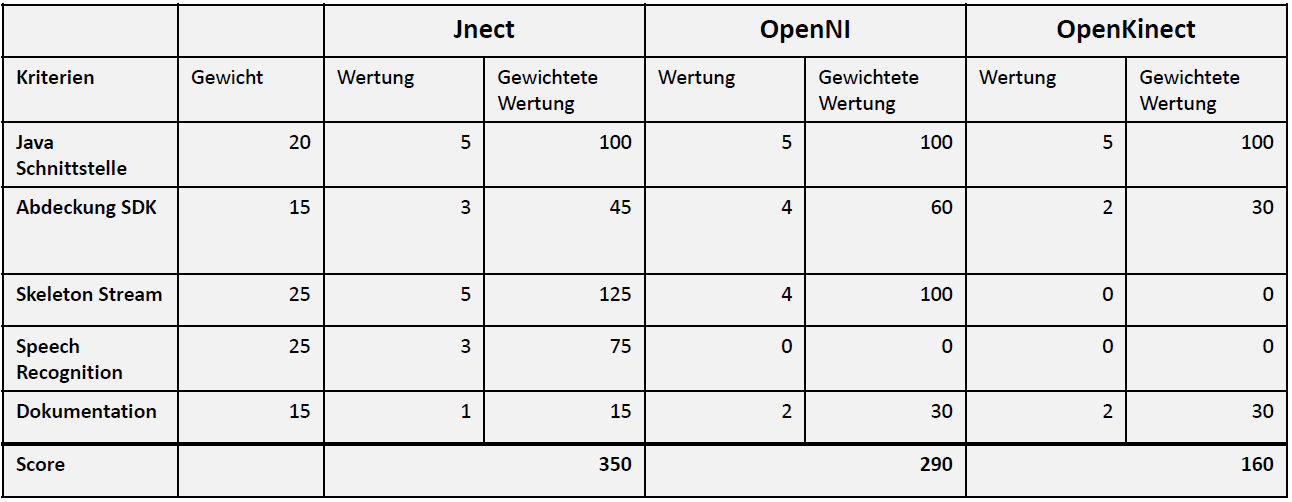
\includegraphics[width=0.9\textwidth]{img/04kapitel/nutzwert.png}
\caption[Nutzwertanalyse Frameworks]{Nutzwertanalyse der verwendbaren Frameworks}
\label{fig:nutzwert}
\end{figure}

Da weder bei OpenKinect noch bei OpenNI eine Spracherkennung enthalten ist, diese sehr schlecht abschneiden. Zwar h\"Atte man sich im Notfall einer Umgehungsl\"osung, wie das entwickeln eigener Treiber, widmen k\"onnen, jedoch h\"Atte dies die Durchf\"uhrbarkeit des Projekts gef\"Ahrdet. Ein Problem mit allen Frameworks ist es, dass sie nur sehr schlecht dokumentiert sind.

\subsection{Analyseergebnis}
%Resultat: jnect \ldots das beste vom besten

Aufgrund der guten Eignung wird f\"ur die Umsetzung dieser Arbeit auf das Projekt jnect gesetzt, wie im Ergebnis der Analyse in Abbildung~\ref{fig:nutzwert} zu sehen.
Zwar werden die Anforderungen nicht vollumfanglich erf\"ullt, jedoch in jeweils ausreichendem Ma\ss e. 